\documentclass[12pt]{article}

% Idioma y codificación
\usepackage[utf8]{inputenc}
\usepackage[spanish]{babel}
\addto\captionsspanish{\renewcommand{\abstractname}{Abstract}}

% Márgenes
\usepackage{geometry}
\geometry{a4paper, left=2.5cm, right=2.5cm, top=2.5cm, bottom=2.5cm}

% Imágenes
\usepackage{graphicx}

% Matemática (solo si planeas usarla)
\usepackage{amsmath}
\usepackage{amssymb}

% Enlaces
\usepackage[colorlinks=true,
linkcolor=blue,
citecolor=blue,
urlcolor=blue]{hyperref}

\begin{document}
	
	\begin{titlepage}
		\centering
		
		\vspace*{-1cm}
		
\includegraphics[width=4cm]{Photos/matcom.jpeg}
		\vspace{1cm}
		
		{\Large \textbf{Universidad de La Habana}}\\[0.3cm]
		{\large \textbf{Facultad de Matemática y Computación}}\\[1cm]
		
		{\large Asignatura: Historia de la Computación}\\[2cm]
		
		{\LARGE \textbf{La evolución de los lenguajes de programación}}\\[0.8cm]
		
		{\Large \textbf{Integrantes}}\\[0.6cm]
		{\large Jabel Resendiz Aguirre}\\
		{\large Noel Pérez Calvo}\\
		
		{\large Carrera: Ciencia de la Computación}\\[2cm]
		
		\vfill
		{\large \today}
	\end{titlepage}

\begin{abstract}
	Este informe presenta un análisis exhaustivo de la evolución de los lenguajes de programación, estructurado a través de las cinco generaciones que definen el incremento en los niveles de abstracción respecto al hardware. Se examinan los antecedentes teóricos del Plankalkül y la transición de los lenguajes de bajo nivel (1GL y 2GL) hacia los pioneros de alto nivel como FORTRAN, LISP y COBOL. Se destaca de manera particular el impacto de ALGOL 60 en la introducción de la estructura de bloques y la formalización de la sintaxis mediante la notación Backus-Naur (BNF), hito fundamental para la teoría de lenguajes y el diseño de compiladores. Finalmente, se aborda la consolidación de los paradigmas imperativo, funcional y orientado a objetos, concluyendo con las tendencias actuales en seguridad de memoria y concurrencia representadas por lenguajes como Rust y Go.
\end{abstract}

\noindent \textbf{Palabras clave:} Historia de la computación, lenguajes de programación, niveles de abstracción, paradigmas de programación, BNF, semántica estática, evolución tecnológica.

\vspace{0.8cm}

\section{Los Inicios y la Abstracción del Hardware (1940s–1950s)}

Los primeros años de la computación estuvieron marcados por una estrecha relación entre el software y el hardware, donde la programación se realizaba directamente en lenguaje máquina. Este tipo de lenguaje consiste en secuencias de instrucciones binarias específicas para cada arquitectura, lo que implica una fuerte dependencia del hardware subyacente y una nula portabilidad entre sistemas \cite{sebesta}.

Desde el punto de vista técnico, este enfoque presentaba múltiples limitaciones. En primer lugar, la programación en lenguaje máquina dificultaba la legibilidad y comprensión del código, aumentando significativamente la probabilidad de errores. En segundo lugar, el uso de direccionamiento absoluto obligaba a los programadores a gestionar manualmente las direcciones de memoria, de modo que cualquier modificación en el programa podía requerir la reescritura de múltiples instrucciones \cite{sebesta}.

Además, en esta etapa temprana no existía una separación clara entre los conceptos de lenguaje, implementación y ejecución. Los programas estaban completamente ligados al modelo de arquitectura de von Neumann, donde tanto los datos como las instrucciones compartían el mismo espacio de memoria, lo que condicionaba directamente el diseño de los programas.

Ante estas limitaciones, surgió la necesidad de introducir mecanismos de abstracción que permitieran independizar parcialmente el desarrollo de software respecto al hardware. Este proceso de abstracción constituye uno de los pilares fundamentales en la evolución de los lenguajes de programación, ya que permitió aumentar la productividad, reducir errores y sentar las bases para la creación de lenguajes de alto nivel.

De esta manera, la transición desde el lenguaje máquina hacia representaciones más simbólicas marcó el inicio de una evolución progresiva en los niveles de abstracción, que culminaría en la aparición de los primeros lenguajes de alto nivel a finales de la década de 1950.


\subsection{Plankalkül: El primer lenguaje de alto nivel}

Entre 1943 y 1945, Konrad Zuse desarrolló el lenguaje Plankalkül, considerado el primer lenguaje de programación de alto nivel, aunque nunca fue implementado en su época \cite{sebesta}. Aunque cronológicamente las máquinas con lenguaje máquina (1GL) ya existían y eran utilizadas, Plankalkül constituye un avance conceptual, pues proponía abstraer la programación de los detalles binarios del hardware y describir algoritmos de forma más simbólica y estructurada.Por ejemplo, las primeras máquinas de Zuse, como la Z1, usaban instrucciones binarias que se ejecutaban directamente en el hardware (ver Figura~\ref{fig:z1}), lo que ilustra la complejidad y la baja abstracción de los primeros sistemas \cite{zuse_replica}.
Este lenguaje introdujo conceptos avanzados para su tiempo, incluyendo tipos de datos estructurados como arreglos y registros, además de soporte para números enteros y de punto flotante. A diferencia de los lenguajes de máquina, Plankalkül permitía describir algoritmos de forma más abstracta, separando en cierta medida la lógica del programa de los detalles del hardware subyacente.

\begin{figure}[h]
	\centering
	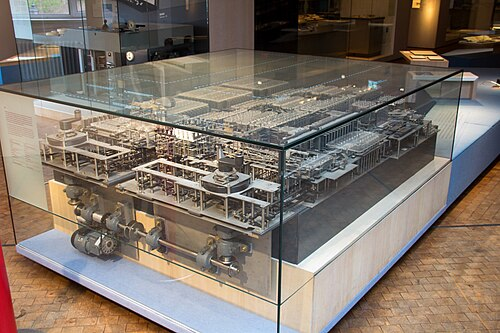
\includegraphics[width=0.7\textwidth]{Photos/z1_replica.jpg}
	\caption{Réplica de la computadora Z1 de Konrad Zuse, mostrando el tipo de instrucciones en lenguaje máquina que se utilizaban en la época.}
	\label{fig:z1}
\end{figure}

Desde el punto de vista técnico, Plankalkül incorporaba ideas que serían fundamentales décadas más tarde en el diseño de lenguajes, como la estructuración de datos complejos y la posibilidad de trabajar con expresiones matemáticas dentro del propio código. Asimismo, incluía mecanismos de control como estructuras iterativas y condicionales, aunque con ciertas limitaciones, como la ausencia de una cláusula \textit{else}. También es notable la inclusión de expresiones que describían propiedades del estado del programa durante su ejecución, anticipando conceptos modernos relacionados con la verificación formal.

Plankalkül permitió la expresión de algoritmos complejos, incluyendo programas para ordenar datos, analizar grafos e incluso jugar ajedrez, lo cual demuestra un nivel de abstracción muy superior al de los lenguajes de máquina \cite{sebesta}. Sin embargo, su notación era extensa y poco intuitiva, ya que cada instrucción podía requerir múltiples líneas para especificar operaciones, índices y tipos de datos, lo que dificultó su comprensión y adopción.

A pesar de no haber sido utilizado en la práctica en su momento, Plankalkül representa un hito fundamental en la historia de los lenguajes de programación, ya que anticipó numerosas características que más tarde serían estándar en los lenguajes de alto nivel. Su escasa difusión, debida en gran medida al contexto histórico de la Segunda Guerra Mundial, limitó su impacto inmediato, aunque su reconocimiento posterior lo posiciona como un precursor clave en la evolución de la programación moderna \cite{sebesta}.

\subsubsection*{Ejemplo de uso: modelando el ajedrez en Plankalkül}

Konrad Zuse utilizó Plankalkül para modelar estructuras complejas, como un juego de ajedrez, demostrando la capacidad del lenguaje para manejar datos compuestos y algoritmos estructurados. A continuación se presenta un ejemplo de cómo se representan coordenadas, piezas y estado del juego:

\begin{table}[h]
	\centering
	\begin{tabular}{|c|c|p{8cm}|}
		\hline
		\textbf{Variable} & \textbf{Notación} & \textbf{Significado} \\
		\hline
		$A_1$ & $S_1 \cdot 3$ & Coordenada de una casilla del tablero (3 bits son suficientes para un tablero de 8x8). \\
		\hline
		$A_2$ & $2 \times A_1$ & Representa una casilla específica en el tablero, por ejemplo L00, 00L (e2). \\
		\hline
		$A_3$ & $S_1 \cdot 4$ & Identificación de una pieza (por ejemplo, 00L0 → rey blanco). \\
		\hline
		$A_4$ & $(A_2, A_3)$ & Una pieza en una casilla concreta (ej. rey blanco en e2). \\
		\hline
		$A_5$ & $64 \times A_3$ & Tablero completo: describe qué pieza está en cada una de las 64 casillas. \\
		\hline
		$A_{10}$ & $(A_5, S_0, S_1 \cdot 4, A_2)$ & Estado completo del juego: tablero, jugador que mueve, posibilidad de enroque y celda para movimiento \textit{en passant}. \\
		\hline
	\end{tabular}
	\caption{Ejemplo de variables en Plankalkül para representar un juego de ajedrez.}
	\label{tab:plankalkul-ajedrez}
\end{table}

\noindent \textbf{Interpretación:} 
\begin{itemize}
	\item Las variables más simples ($A_1$, $A_3$) representan coordenadas y piezas individuales.
	\item Variables compuestas ($A_4$, $A_5$, $A_{10}$) combinan información de varias simples para describir posiciones de piezas, tablero completo y estado del juego.
	\item Este ejemplo muestra cómo Plankalkül permitía abstraer la lógica de un juego completo, sin necesidad de programar en lenguaje máquina.
	\item Permite implementar reglas, movimientos y verificaciones de estado usando únicamente estructuras simbólicas.
\end{itemize}

\noindent Este tipo de ejemplos evidencia la capacidad de Plankalkül de manejar datos complejos y anticipa conceptos modernos de programación estructurada y tipado compuesto.

\subsection{Lenguajes de bajo nivel: 1GL}

Los lenguajes de primera generación (1GL), conocidos como lenguaje máquina, constituyen la forma más básica y primitiva de programación. Estos lenguajes están compuestos por secuencias de instrucciones en formato binario que son directamente ejecutadas por el hardware, sin necesidad de traducción o interpretación adicional \cite{sebesta}. Cada instrucción representa una operación elemental del procesador, como la manipulación de datos, operaciones aritméticas o transferencias de control.

Desde un punto de vista estructural, el lenguaje máquina está completamente ligado a la arquitectura de la computadora. Esto implica que el conjunto de instrucciones, los formatos binarios y los modos de direccionamiento dependen directamente del diseño del procesador, lo que impide la portabilidad del software entre diferentes sistemas \cite{tanenbaum}. En consecuencia, un programa escrito para una máquina específica no puede ejecutarse en otra sin ser reescrito.

Una de las principales dificultades asociadas a estos lenguajes es su baja legibilidad. Las instrucciones se representan mediante códigos numéricos o binarios, lo que dificulta tanto su comprensión como su mantenimiento. A diferencia de los lenguajes modernos, no existen representaciones simbólicas ni estructuras que faciliten la interpretación humana del código \cite{stallings}.

Otro problema fundamental es el uso del direccionamiento absoluto. En este esquema, las instrucciones hacen referencia explícita a posiciones concretas de memoria, lo que complica enormemente la modificación de programas. Por ejemplo, la inserción o eliminación de una instrucción puede requerir la actualización manual de múltiples direcciones, aumentando considerablemente la probabilidad de errores \cite{sebesta}.

Además, los lenguajes de máquina carecen de mecanismos de abstracción. No existen estructuras de control de alto nivel, tipos de datos complejos ni modularidad. El flujo de ejecución debe gestionarse mediante saltos explícitos entre direcciones de memoria, lo que conduce a programas difíciles de seguir y propensos a fallos.

A pesar de estas limitaciones, el lenguaje máquina desempeñó un papel fundamental en los inicios de la computación, ya que permitió el desarrollo de los primeros programas ejecutables y sentó las bases para la evolución posterior de los lenguajes de programación hacia niveles más altos de abstracción.

\begin{figure}[h]
	\centering
	\includegraphics[width=0.7\textwidth]{Photos/Machine_language.png}
	\caption{Ejemplo de instrucciones en Lenguaje de Máquina.}
	\label{fig:maquina}
\end{figure}

\subsection{Pseudocódigos e intérpretes}

Paralelamente al desarrollo de los lenguajes ensambladores, a finales de los años 40 y principios de los 50 surgieron los llamados pseudocódigos, que representaron uno de los primeros intentos de simplificar y automatizar la programación. Aunque el término difiere de su significado actual, en este contexto se refería a sistemas que permitían expresar operaciones mediante representaciones simbólicas más cercanas a la notación matemática que al lenguaje máquina \cite{sebesta}.

Estos lenguajes surgieron como respuesta a las limitaciones del código máquina, particularmente su complejidad y falta de herramientas de apoyo. En una época donde no existían compiladores ni entornos de desarrollo, los pseudocódigos introdujeron una capa intermedia que facilitaba la escritura de programas, especialmente en aplicaciones científicas que requerían cálculos numéricos complejos.

Uno de los más importantes fue el \textit{Short Code}, desarrollado en 1949, que permitía expresar operaciones matemáticas mediante códigos simbólicos que eran posteriormente interpretados por la máquina \cite{sebesta}. Este enfoque reducía considerablemente el esfuerzo de programación, ya que los programadores podían trabajar con expresiones más cercanas al razonamiento matemático.

Sin embargo, estos sistemas no eran compilados, sino interpretados, lo que implicaba que cada instrucción debía ser traducida en tiempo de ejecución. Como consecuencia, el rendimiento era significativamente inferior al del lenguaje máquina; por ejemplo, el Short Code podía ser hasta 50 veces más lento \cite{sebesta}. Esta desventaja reflejaba una de las primeras manifestaciones del compromiso entre facilidad de programación y eficiencia de ejecución.

Otro avance relevante fue el sistema \textit{Speedcoding}, desarrollado por John Backus en 1954, que transformaba la computadora IBM 701 en una especie de calculadora de punto flotante mediante un intérprete \cite{backus1953}. Este sistema incorporaba operaciones avanzadas como suma, multiplicación, raíz cuadrada, funciones trigonométricas, exponencial y logaritmo, así como mecanismos de manejo de arreglos y bloques de datos. Además, Speedcoding ofrecía facilidades para la entrada y salida de información, comprobaciones automáticas de errores y modificación automática de direcciones, simplificando la programación y verificación de programas complejos. Aunque la ejecución era más lenta que en código máquina, el sistema reducía drásticamente el tiempo de desarrollo: problemas que podrían requerir semanas en lenguaje máquina podían resolverse en unas pocas horas \cite{backus1953, sebesta}.

En conjunto, los pseudocódigos y los sistemas interpretados marcaron un paso intermedio clave en la evolución de los lenguajes de programación, al introducir un mayor nivel de abstracción y demostrar que era posible automatizar parcialmente la traducción de instrucciones, sentando así las bases para el desarrollo posterior de compiladores y lenguajes de alto nivel.

\begin{figure}[h]
	\centering
	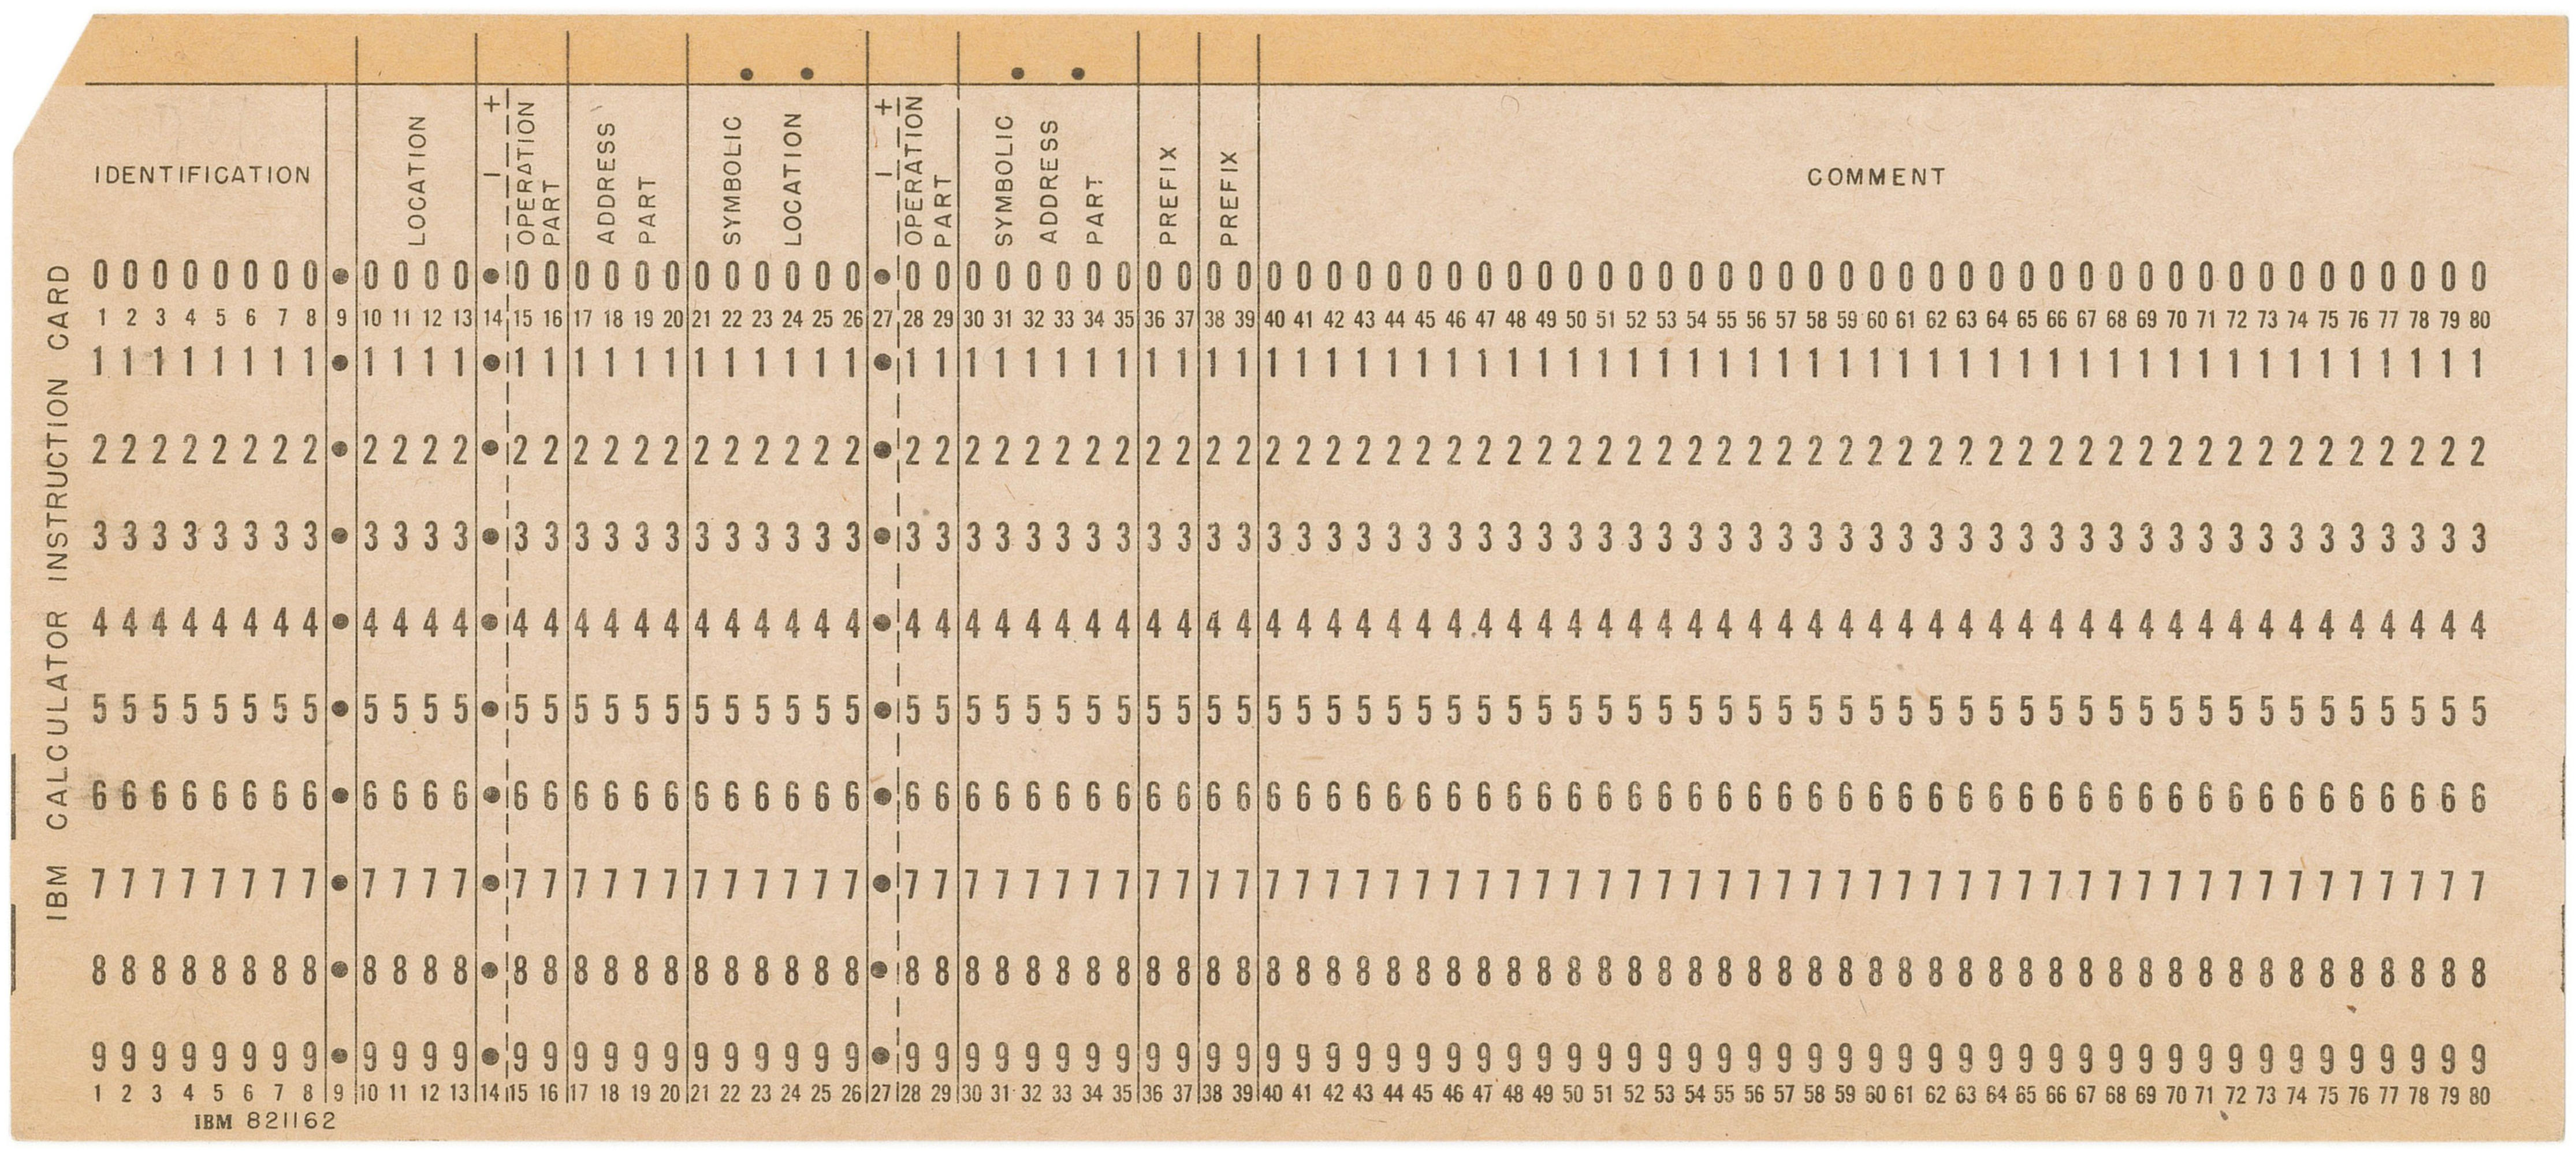
\includegraphics[width=0.7\textwidth]{Photos/punched_card.jpg}
	\caption{Tarjeta perforada utilizada para ingresar programas como Short Code o Speedcoding en las primeras computadoras.}
	\label{fig:punched_card}
\end{figure}

\begin{figure}[h]
	\centering
	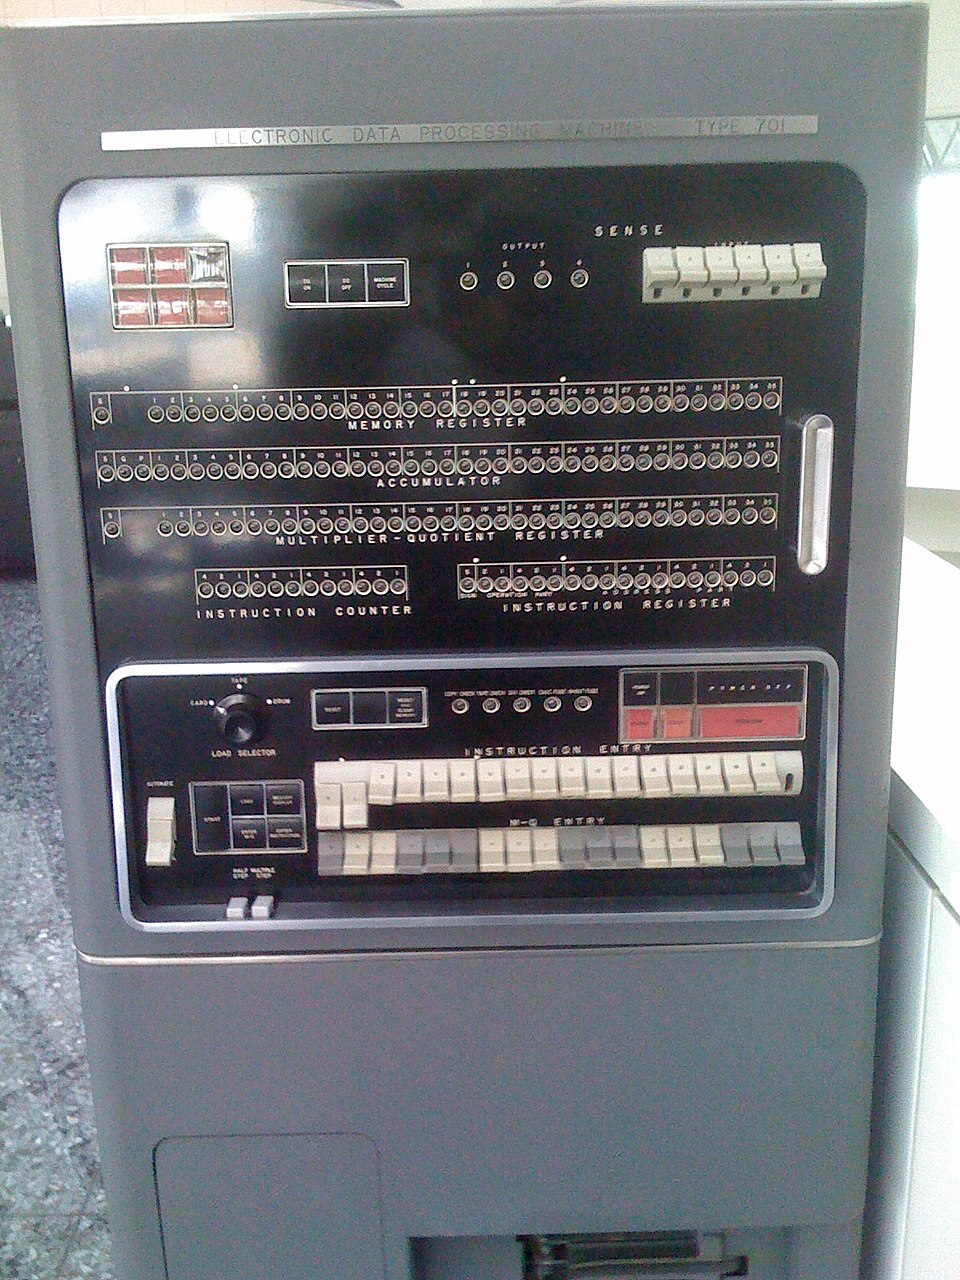
\includegraphics[width=0.7\textwidth]{Photos/ibm701_console.jpg}
	\caption{Panel frontal de la IBM 701, computadora para la que se desarrolló el sistema Speedcoding.}
	\label{fig:ibm701}
\end{figure}

\subsection{Lenguajes de bajo nivel: 2GL}

Las limitaciones inherentes al lenguaje máquina, particularmente su baja legibilidad, la complejidad del direccionamiento absoluto y la alta propensión a errores, motivaron el desarrollo de mecanismos que facilitaran la programación sin alejarse completamente del hardware. En este contexto surgieron los lenguajes de segunda generación (2GL), conocidos como lenguajes ensambladores.

Los lenguajes ensambladores introdujeron una representación simbólica de las instrucciones de máquina mediante el uso de mnemónicos, como \texttt{ADD}, \texttt{MOV} o \texttt{JMP}, que reemplazaban los códigos binarios o numéricos. Esta transformación permitió mejorar significativamente la legibilidad del código, facilitando tanto su escritura como su comprensión \cite{sebesta}.

Además, los ensambladores incorporaron el uso de etiquetas simbólicas para referirse a direcciones de memoria, lo que eliminó en gran medida la necesidad de gestionar manualmente el direccionamiento absoluto. Esto simplificó la modificación de programas y redujo la probabilidad de errores asociados a cambios en el código \cite{tanenbaum}.

Desde el punto de vista funcional, los lenguajes ensambladores mantenían una correspondencia casi directa con las instrucciones del hardware, lo que garantizaba un control preciso sobre los recursos del sistema. Sin embargo, a diferencia del lenguaje máquina, estos lenguajes requerían de un programa traductor, denominado ensamblador, que convertía el código simbólico en instrucciones binarias ejecutables por la máquina \cite{stallings}.

A pesar de estas mejoras, los lenguajes de segunda generación continuaban siendo dependientes de la arquitectura del sistema, ya que cada tipo de procesador posee su propio conjunto de instrucciones. En consecuencia, los programas escritos en ensamblador no eran portables entre diferentes máquinas sin modificaciones significativas.

En términos históricos, los lenguajes ensambladores representaron un avance crucial en la evolución de la programación, al introducir un primer nivel de abstracción que permitió a los programadores centrarse más en la lógica del programa que en los detalles binarios, sentando así las bases para el desarrollo de lenguajes de más alto nivel.


\begin{figure}[h]
	\centering
	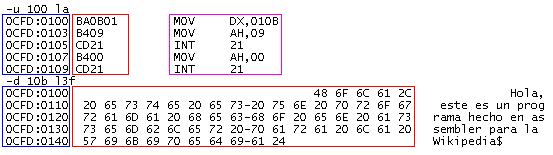
\includegraphics[width=0.7\textwidth]{Photos/Codigo_de_maquina.png}
	\caption{Ejemplo de instrucciones en Lenguaje Ensamblador.}
	\label{fig:ensamblador}
\end{figure}

\subsection{Hacia la abstracción del hardware}

Los desarrollos descritos marcaron el inicio de un cambio fundamental en la computación: la transición desde una programación completamente dependiente del hardware hacia un enfoque basado en niveles crecientes de abstracción. Este cambio no solo implicó una mejora en la forma de escribir programas, sino también una transformación en la manera de concebir el software, separando progresivamente la lógica del programa de los detalles físicos de la máquina \cite{sebesta}.

Aunque los primeros sistemas, como los pseudocódigos y los intérpretes, eran considerablemente ineficientes en términos de rendimiento, demostraron que era posible simplificar la programación mediante la introducción de representaciones intermedias. Este avance evidenció que la productividad del programador podía incrementarse significativamente sin necesidad de interactuar directamente con el lenguaje máquina, estableciendo así un nuevo paradigma en el desarrollo de software.

En este contexto, comenzó a consolidarse la idea de automatizar completamente la traducción de programas, lo que conduciría al desarrollo de los primeros compiladores. Este proceso sentó las bases para la aparición de los lenguajes de alto nivel en la década de 1950, como FORTRAN y LISP, los cuales transformarían de manera definitiva la programación al introducir estructuras más expresivas, portabilidad y una mayor independencia del hardware.

\bibliographystyle{plain} .
\bibliography{referencias} 

\end{document}